% This is the main LaTeX file which is used to produce the Biopython
% Tutorial documentation.
%


\documentclass{report}
\usepackage{url}
\usepackage{fullpage}
\usepackage{hevea}
\usepackage{graphicx}

% make everything have section numbers
\setcounter{secnumdepth}{4}

% Make links between references
\usepackage{hyperref}
\newif\ifpdf
\ifx\pdfoutput\undefined
  \pdffalse
\else
  \pdfoutput=1
  \pdftrue
\fi
\ifpdf
  \hypersetup{colorlinks=true, hyperindex=true, citecolor=red, urlcolor=blue}
\fi

\begin{document}

\begin{htmlonly}
\title{Gene Ontology package to Biopython Tutorial}
\end{htmlonly}
\begin{latexonly}
\title{
%Hack to get the logo on the PDF front page:
\includegraphics[width=\textwidth]{images/biopython.jpg}\\
%Hack to get some white space using a blank line:
~\\
Gene Ontology package to Biopython}
\end{latexonly}

\author{Kamil Koziara}
\date{Last Update -- 3 September 2016 (Biopython 1.63b+)}

%Hack to get the logo at the start of the HTML front page:
%(hopefully this isn't going to be too wide for most people)
\begin{rawhtml}
<P ALIGN="center">
<IMG ALIGN="center" SRC="images/biopython.jpg" TITLE="Biopython Logo" ALT="[Biopython Logo]" width="1024" height="288" />
</p>
\end{rawhtml}

\maketitle
\tableofcontents

% Bio.Ontology

\chapter{Ontology analysis with Bio.Ontology}

\label{sec:Ontology}

With huge amount of information from biological experiments the problem of
getting the right answers from them is growing bigger. Ontologies are
vocabularies created to unify the representation of terms across different
biological and medical domains. With annotations they provide means for
interpretation of experiments, so that collected data gains a meaning.

The Bio.Ontology package is a tool which helps to get the most of the
Ontologies in a convenient manner. It provides a set of tools for reading
and processing ontologies and a handful of tools for presenting the obtained
results in readable form.

\section{Ontology - what's in it?}
\label{sec:demo}

To get more understanding of what you can do with Bio.Ontology let's start with
a simple case study, which will serve as an introduction to processing
biomedical data with ontologies. 

Let's assume we carried out an experiment and got data about gene expression -
a list of genes that are on or in other words their expression level is
siginificant. Now, we would like to get the
information about the biological terms which are connected to obtained pattern
of expression. In the demo we will use the real world data and Drosophila anatomy and development ontology.
\footnote{\url{http://svn.code.sf.net/p/fbbtdv/code/fbbt/releases/fbbt.obo}}

First you need to read the list of genes or type them manually and store as
a list. In our case list represents genes connected to a specific transcription
factor in a specific point in time during the Drosophila mesodrem tissues development.
Let's read the data from a file. The file contains one gene per line.

\begin{verbatim}
>>> with open("tin_l_gene_ids.txt", "r") as my_file:
...    genes_to_study = [x.strip() for x in my_file]

\end{verbatim}

The next important step is obtaining files with gene ontology and gene
associations.

Gene ontology has a form of directed graph.
The most recent ontology in obo format can be downloaded from
\url{http://www.geneontology.org}. Obo format can be easily read using
\verb|Bio.Ontology.IO| module:

\begin{verbatim}
>>> import Bio.Ontology.IO as OntoIO
>>> go_graph = OntoIO.read("fbbt.obo", "obo")
\end{verbatim}

\verb|read| method first argument is path to file (or file handle) and the
second argument is file type. In this case method returns \verb|OntologyGraph|
object which contains the ontolgy representation as directed graph.

Terms in ontology graph are connected by many different relationships. You can
list them by calling \verb|get_relationship_types| method of \verb|OntologyGraph|.
Some of them are not relevant to the study we want to conduct. Therfore we will
call \verb|trim| method, which removes all relationships with type different
than listed.

\begin{verbatim}
>>> g = g.trim(['is_a', 'regulates', 'contained_in',
...     'occurs_in', 'connected_to', 'negatively_regulates',
...     'expresses', 'overlaps', 'part_of', 'partially_overlaps',
...     'positively_regulates',  'located_in'])
\end{verbatim}

Gene association files can be read as easily:

\begin{verbatim}
>>> assocs = OntoIO.read("insitu_annot.tsv", "gaf")
\end{verbatim}


In this case method returns a Python dictionary mapping genes to
annotation objects.

In case study I use associations from \url{http://insitu.fruitfly.org/insitu-mysql-dump/insitu_annot.csv.gz}
which were transformed to commonly used gaf file format.

Now is the time to create \verb|EnrichmentFinder|. In this case we will
use \verb|ParentChildEnrichmentFinder| which implements one of the methods
for finding enrichments called - \emph{parent-child}. Besides the arguments
mentioned before you could specify an id resolver, which basically tries
to find synonyms for gene ids that finder can understand, and population
of genes as reference. If none of this is specified default resolver
is used and all genes from association are used as the population.

\begin{verbatim}
>>> from Bio.Ontology import ParentChildEnrichmentFinder
>>> ef = ParentChildEnrichmentFinder(assocs, go_graph)
\end{verbatim}

Additionally you can specify a list of statistical corrections for multiple
hipothesis testing which should be used (by default the list is empty):

\begin{verbatim}
>>> corrections = ['bonferroni', 'bh_fdr']
\end{verbatim}

Now to run a finder you just need to call \verb|find_enrichment| method with list
of genes as an argument and optionally: a list of corrections and argument
setting a way in which the parents genes will be computed. By default the method
is \verb|"intersection"|. 

\begin{verbatim}
>>> result = ef.find_enrichment(genes_to_study, corrections, method =  "union")
\end{verbatim}

The result is \verb|Enrichment| which contains a list of \verb|EnrichmentEntry|
instances - each for a node in graph which is enriched - and a list of warnings.

\begin{verbatim}
>>> print result
Enrichment found using parent_child_union method: 186 entries, 0 warnings.
\end{verbatim}

We found 186 enriched terms and there is no warnings. Warnings may contain
information about resolved gene names or cycles found in the graph.

You may want to specify the significance level and filter out only results
equally or more significant. To do this you call \verb|filter_p_val| method
of \verb|Enrichment| with significance level as an argument:

\begin{verbatim}
>>> significant_result = result.filter_p_val(0.01)
>>> print significant_result
Enrichment found using parent_child_union method: 13 entries, 0 warnings.
\end{verbatim}


The standard entry representation looks as follows:

\begin{verbatim}
>>> print significant_result.entries[0]
ID : FBbt:00007003
name : portion of tissue
p-value : 0.00087718387734
corrected p-values: {'bh_fdr': 0.07131507455039117, 'bonferroni': 0.1631562011852869}
\end{verbatim}

There are a few ways of representing the result in a graphical form - all
contained in \verb|PrettyIO| module and accessible from Ontology module by
calling \verb|pretty_print| method. First argument is enrichment, the
second one is graph with ontology, third - the filename and fourth is
representation type. \verb|"png"| is output to png file using GraphViz through
\verb|pygraphviz| module (which has to be installed for this functionality to
work).

\begin{verbatim}
>>> import Bio.Ontology.IO as OntoIO
>>> OntoIO.pretty_print(significant_result, go_graph, "tin_l_gene_ids.png", "png")
\end{verbatim}

The output looks as in Figure~\ref{fig:graphoutput}. As you can see in this example
the gene expression pattern is tightly connected with development of 
mesoderm tissues and muscle primodia which is exactly what you would expect
because of the data source.

\begin{htmlonly}
\label{fig:graphoutput}
\imgsrc{images/tin_l_gene_ids.png}
\end{htmlonly}

\begin{latexonly}
\begin{figure}[htbp]
\centering
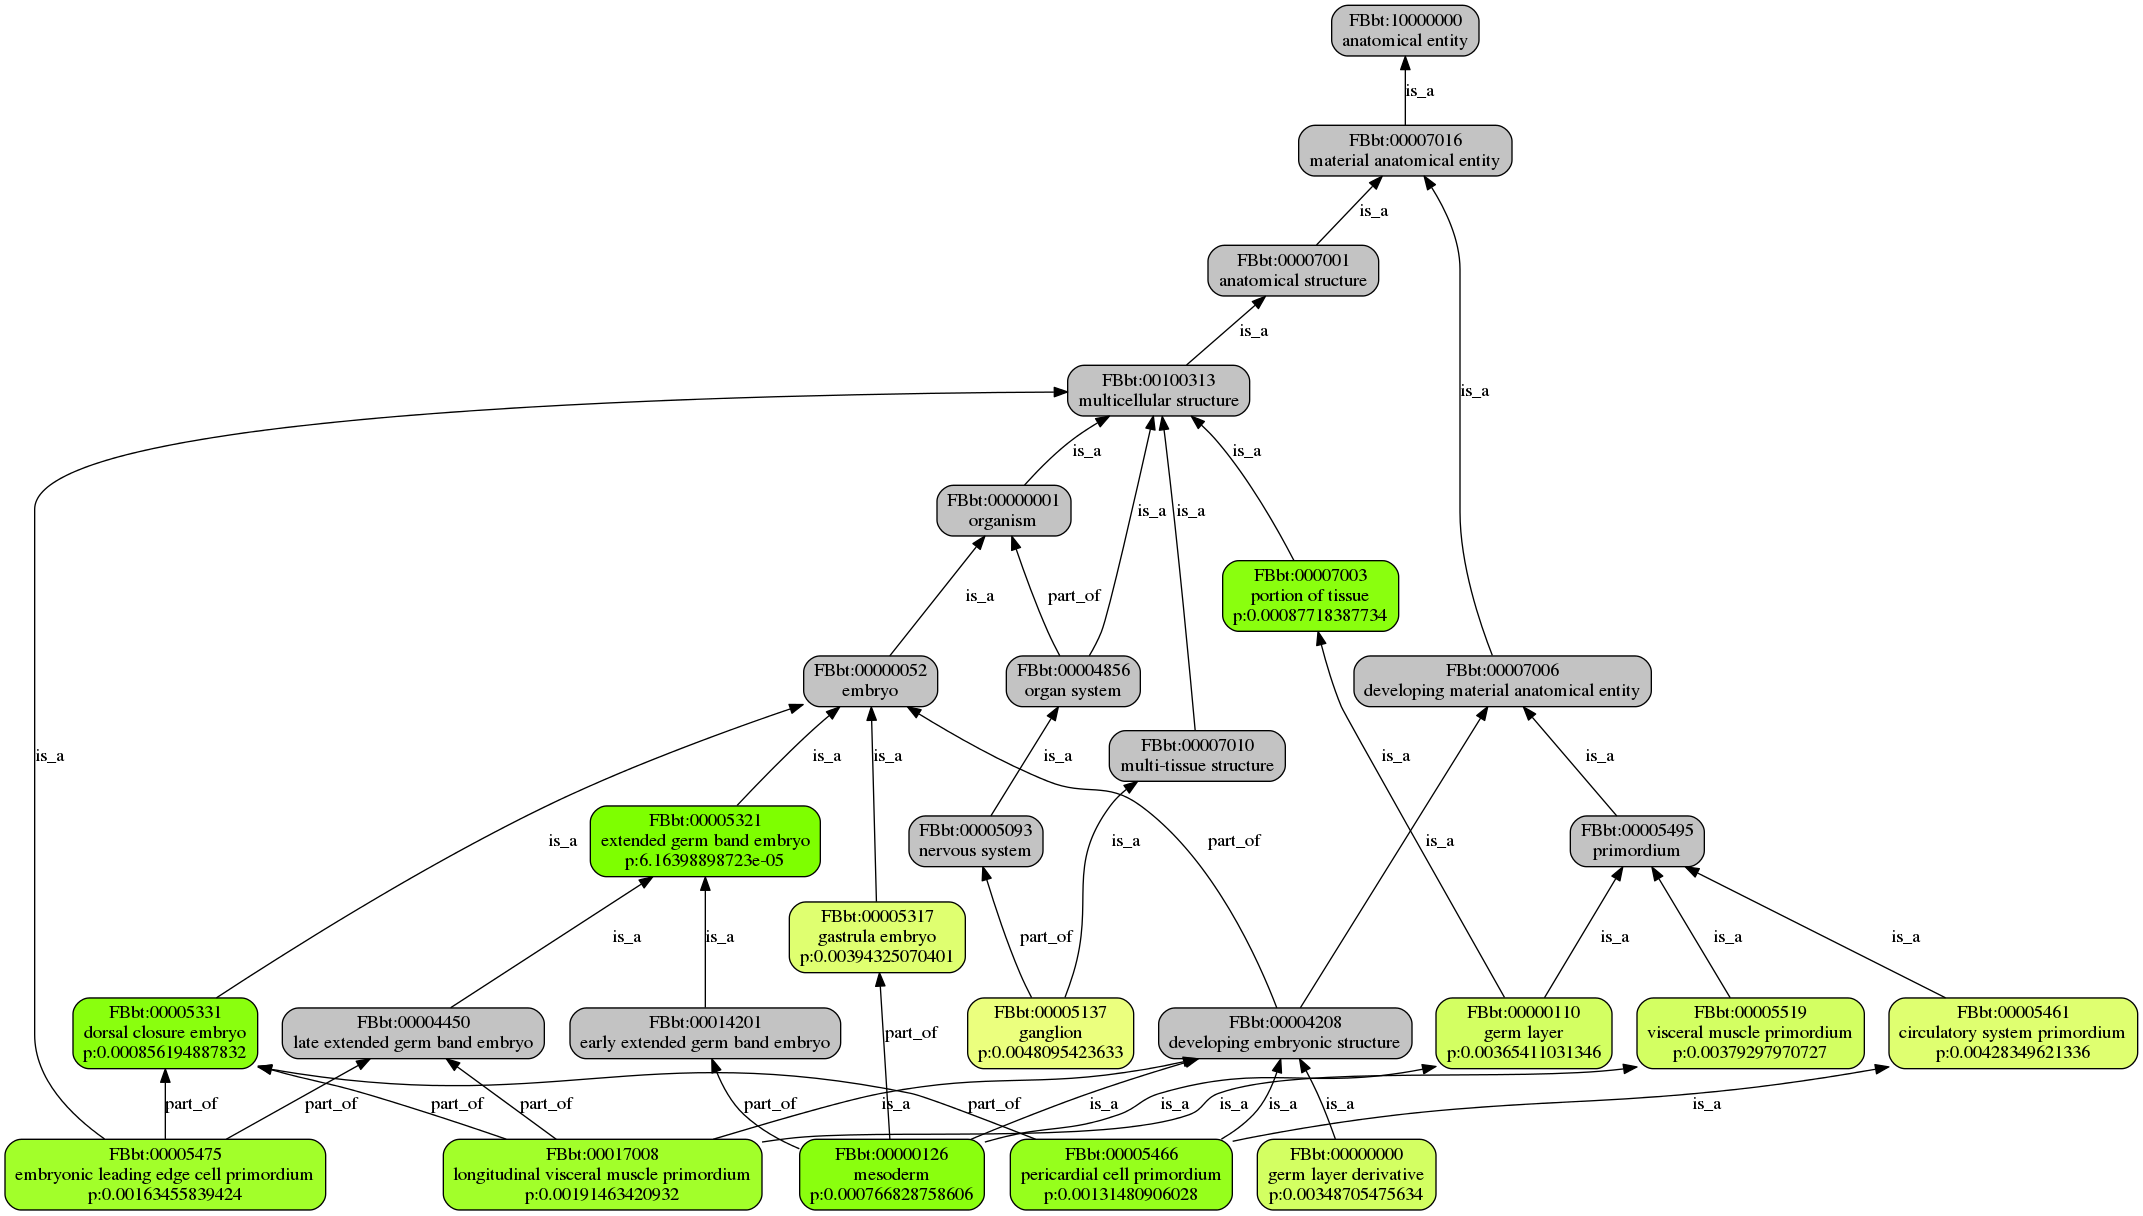
\includegraphics[width=0.8\textwidth]{images/tin_l_gene_ids.png}
\caption{Enrichment representation as a graph.}
\label{fig:graphoutput}
\end{figure}
\end{latexonly}

\section{I/O functions}

Bio.Ontology module conforms with most of the BioPython toolkit if it comes to
I/O functions: after importing \verb|Bio.Ontology.IO| module you can call its
\verb|read|, \verb|write| and \verb|parse| methods to
perform various input / output operations.

\verb|parse| method takes file name (or file handle) and file type as arguments
and returns iterator to objects stored in it.
Supported file types are:
\begin{itemize}
%\item \verb|"gaf"| - GO Annotation File Format\footnote{More detailed description
%can be found at \url{http://www.geneontology.org/GO.format.gaf-2_0.shtml}}
%which stores information about genes to terms annotations.
%Returned value is map from Gene Ids to \verb|GeneAnnotation| objects.
\item \verb|"tsv"| - text files in which each row containes tab separated values. Returned
value is iterator to list of row fields.
\item \verb|"obo"| - text file format used for storing ontologies. \footnote{More details at
\url{http://www.geneontology.org/GO.format.shtml}}
Returned value is iterator to pairs of two types: either
\verb|("Term", node_of_the_graph)| or \verb|("Typedef", relation_type_definition)|.
\end{itemize}

\verb|read| method takes file name (or file handle) and file type as arguments.
Additionally for some of the file types you can specify named arguments.
Supported file types are:
\begin{itemize}
\item \verb|"nexo"| - xgmml file containing ontology graph with gene / orfs
annotations created by Nexo software.\footnote{More details at \url{http://www.nexontology.org/}}
Additional arguments are:
\begin{itemize}
\item \verb|annotation_source| - states whether we want to use genes (\verb|"genes"|)
or orfs (\verb|"orfs"|) as the annotations.
\item \verb|get_all_attrs| - if set to \verb|True| it reads additional terms attributes
from the nexo file.
\end{itemize}
Returns pair containing list of annotations and \verb|OntologyGraph|. 
\item \verb|"obo"| - GO Annotation File Format. Returns
\verb|OntologyGraph|.
\item \verb|"gaf"| - GO Annotation File Format\footnote{More detailed description
can be found at \url{http://www.geneontology.org/GO.format.gaf-2_0.shtml}}
which stores information about annotations of genes to ontology terms.
Returned value is map from gene ids to \verb|GeneAnnotation| objects.
Depending on value of parameter \verb|assoc_format| map might be:
\begin{itemize}
\item \verb|"dict"| - standard Python dictionary. It is fast but
gives about 700\% memory overhead.
\item \verb|"in_mem_sql"| - \verb|InSqlAssoc| object with
dictionary-like interface. It is immutable in memory sql database, which
is slower than the dictionary but the memory overhead is only 25\%, so its use might be necessary for large gaf files.
\end{itemize}
\item \verb|"etsv"| - format used for storing information about
enrichments. For more information see \ref{ch:fileformats}. Returned
value is \verb|Enrichment| object. Additional argument is
\verb|read_attrs| - if \verb|True| additional information stored
in enrichments are read.
\end{itemize}

\verb|write| method takes object with data, file name (or file handle) and file
type as arguments. You can also specify additional arguments.
Supported file types are:
\begin{itemize}
% \item "obo" - very basic writer of obo files (not finished). As an additional
% argument you should specify version of obo file.
% \item "gml" - writes \verb|DiGraph| to gml file. It is used by \verb|pretty_print| to
% write out results to gml files. 
\item \verb|"etsv"| - format used for storing information about
enrichments. Additional argument is
\verb|write_attrs| - if \verb|True| additional information stored
in enrichments are written.

\item \verb|"png"| - writes \verb|OntologyGraph| to image in png format. The
\verb|pygraphviz| package must be installed for this feature to work. As an
additional argument you can specify dpi and nodes color, though it is not
necessary.
\begin{verbatim}
>>> import Bio.Ontology.IO as OntoIO
>>> OntoIO.write(graph, "graph.png", dpi = 96, color = "#00bd28")
\end{verbatim}

\end{itemize}
\section{File types}
\label{ch:fileformats}
This section contains information about file types introduced with
Bio.Ontology module.
\subsection{etsv}
\verb|etsv| format was created to allow for exporting computed
\verb|Enrichment| objects.
The structure of the file is as follows:
\begin{itemize}
\item In the first row after \verb|#| the name of the method used
to compute enrichment is given,
\item Next line consist of \verb|#| and two numbers: $x$ - number of 
enriched terms and $y$ - number of warnings,
\item Third rows contains labels of attributes of
\verb|EnrichmentEntry|:
\begin{itemize}
\item id
\item name
\item p-value
\item names of corrections for multiple hypothesis testing separated by
$|$ sign
\item attrs - additional attributes
\end{itemize}
\item $x$ rows for each enriched term,
\item $y$ rows for each warning.
\end{itemize}

\begin{verbatim}
# GSEA
# 825 1
id    name                                  p-value   fdr   attributes
9075  microtubule organizing center part    0.327     1.0
6168  protein disulfide isomerase activity  0.083     1.0
.
.
.
! Cycles found 
\end{verbatim}

\section{Data structures}
Data read from various files need to be stored somewhere. With many different
types of input Bio.Ontology module provides uniform way of accessing it. In this
section we will focus on data structures you will stumble upon while working
with ontologies.

\subsection{OntologyGraph}
\verb|OntologyGraph| placed in \verb|Bio.Ontology.Data| module provides means
to process and view any ontology graph read into the program. It is a subclass
of more generic \verb|DiGraph| structure for directed graph representation.

Every node in the graph contains \verb|OntologyTerm| instance. \verb|OntologyTerm|
has always \verb|id| and \verb|name|. In addition additional attributes are
stored in \verb|attrs|

Interesting methods of \verb|OntologyGraph| include:
\begin{itemize}
\item \verb|get_term(id)| - returns term with given id,
\item \verb|get_ancestors(id)| - returns terms ancestors,
\item \verb|get_parents(id)| - returns terms parents,
\item \verb|get_relationship_types()| - returns types of relationships between
nodes that can be found in the graph,
\item \verb|trim(relation_list)| - returns graph crated by removing all edges
which types are not present in \verb|relation_list|.
\item \verb|get_induced_subgraph(nodes_ids)| - returns graph created from only
the nodes with ids given in \verb|nodes_ids| argument.
\item \verb|to_networkx(annotations)| - returns networkx graph
containing the information from \verb|OntologyGraph|. If optional map
from ontology terms to genes is given, annotated terms will be
stored in networkx graph as well.
\end{itemize}

Let's assume we have graph like the one on Figure~\ref{fig:ontofullgraph}, and
call some methods to get ancestors and parents of one of the terms:

\begin{verbatim}
>>> print g.get_ancestors("FBbt:00004208")
set(['FBbt:00000001', 'FBbt:00007006', 'FBbt:00007016', 'FBbt:00100313',
     'FBbt:10000000', 'FBbt:00000052', 'FBbt:00007001'])
>>> print g.get_parents("FBbt:00004208")
set(['FBbt:00007006', 'FBbt:00000052'])
\end{verbatim}

Let's trim the graph by leaving only \verb|is_a| edges:
\begin{verbatim}
>>> gtrimmed = g.trim(["is_a"])
>>> OntoIO.write(gtrimmed, "trimmed_g.png", "png")
\end{verbatim}

The output looks like the graph on Figure~\ref{fig:ontotrimmedgraph}.

Now let's get the graph induced by list of nodes:
\begin{verbatim}
>>> ginduced = g.get_induced_subgraph(['FBbt:00000125', 'FBbt:00000126',
...    'FBbt:00000110','FBbt:00004208', 'FBbt:00005495', 'FBbt:00007006'])
>>> OntoIO.write(ginduced, "induced_g.png", "png")
\end{verbatim}

The output looks like the graph on Figure~\ref{fig:ontoinducedgraph}.


\begin{htmlonly}
\label{fig:ontofullgraph}
\imgsrc{images/full_g.png}
\end{htmlonly}

\begin{latexonly}
\begin{figure}[htbp]
\centering
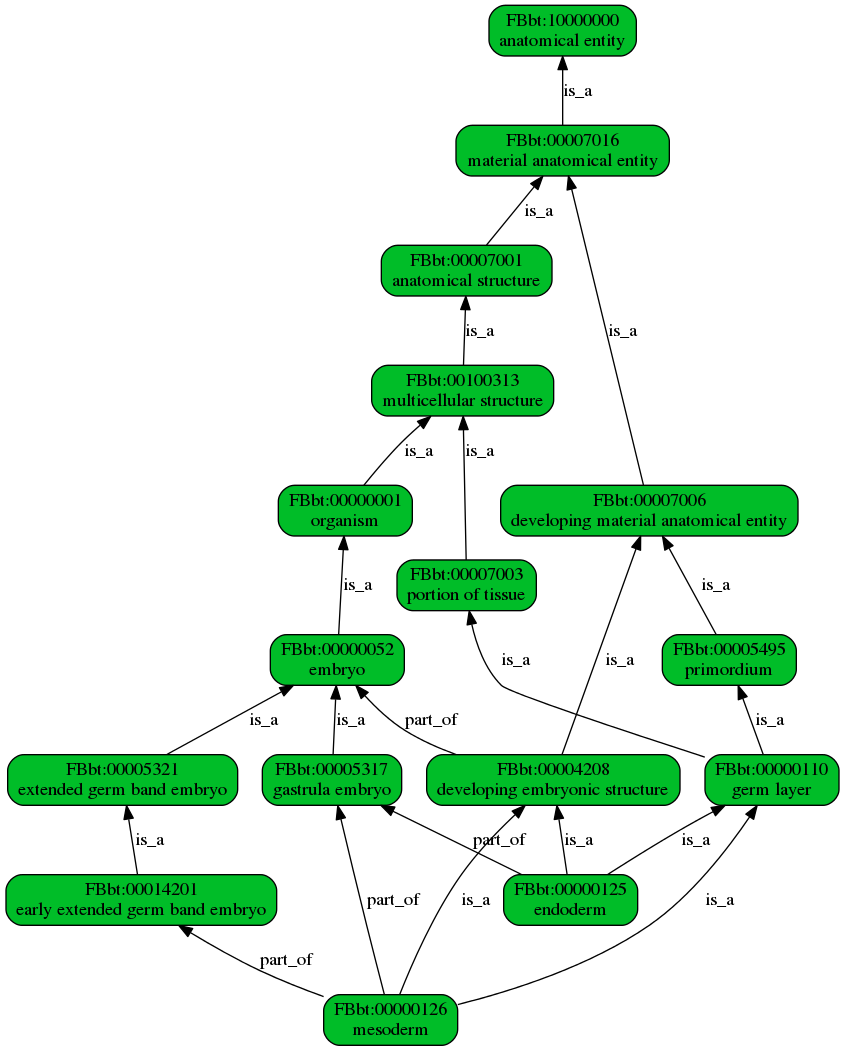
\includegraphics[width=0.6\textwidth]{images/full_g.png}
\caption{Full g graph.}
\label{fig:ontofullgraph}
\end{figure}
\end{latexonly}

\begin{htmlonly}
\label{fig:ontotrimmedgraph}
\imgsrc{images/trimmed_g.png}
\end{htmlonly}

\begin{latexonly}
\begin{figure}[htbp]
\centering
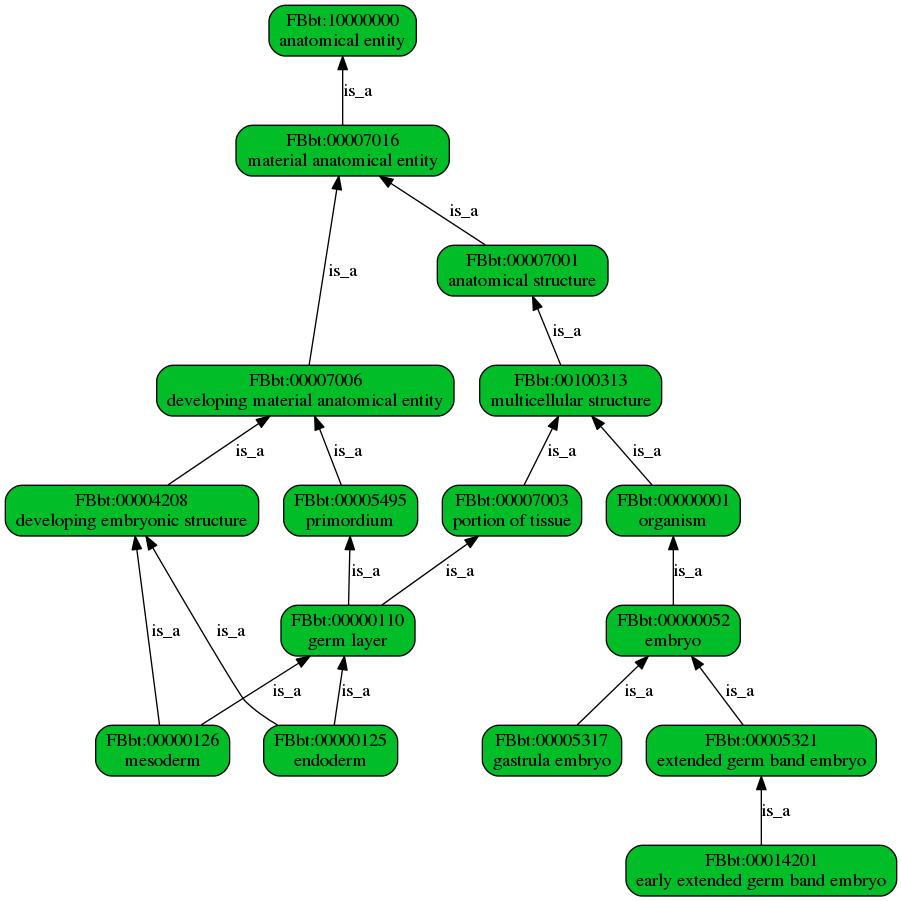
\includegraphics[width=0.6\textwidth]{images/trimmed_g.png}
\caption{Trimmed g graph.}
\label{fig:ontotrimmedgraph}
\end{figure}
\end{latexonly}

\begin{htmlonly}
\label{fig:ontoinducedgraph}
\imgsrc{images/induced_g.png}
\end{htmlonly}

\begin{latexonly}
\begin{figure}[htbp]
\centering
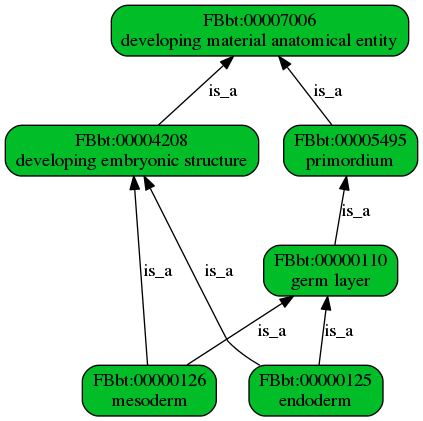
\includegraphics[width=0.3\textwidth]{images/induced_g.png}
\caption{Graph induced by list of nodes from g.}
\label{fig:ontoinducedgraph}
\end{figure}
\end{latexonly}


\subsection{GeneAnnotation and TermAssociation}

\verb|GeneAnnotation| object stores ids of terms annotated to a gene.
Its attributes are:
\begin{itemize}
\item \verb|id| - identifier of gene,
\item \verb|associations| - list of \verb|TermAssociation| objects,
\item \verb|attrs| - additional attributes as Python dict.
\end{itemize}

\verb|TermAssociation| represents gene to term association.
Its attributes are:
\begin{itemize}
\item \verb|term_id|
\item \verb|attrs| - additional attributes as Python dict.
\end{itemize}

\subsection{Enrichment and EnrichmentEntry}
Results of statistical analysis are stored in \verb|Enrichment| object. It
contains list of enriched entries, list of warnings, name of the used method
and list of applied corrections.

\verb|Enrichment| has methods for filtering entries:
\begin{itemize}
\item \verb|filter_p_val(p_val)| - this method returns new \verb|Enrichment|
object with only these entries that have p-value less than \verb|p_val|.

\item \verb|filter(filter_fun)| - this method is more generic. It takes
a function returning True or False which is applied to every entry. Only entries
for which it returned True are left in new \verb|Enrichment| object.

Let's see an example. Assuming we found an enrichment and it has 168 entries:
\begin{verbatim}
>>> e = finder.find_enrichment(gene_list, ["bonferroni", "bh_fdr"],
...                            method =  "parent_child_union")
>>> print e
Enrichment found using parent_child_union method: 168 entries, 0 warnings.
\end{verbatim}
We want only the significant results so now we will filter only the values
with FDR corrected p-value smaller than 0.05:
\begin{verbatim}
>>> e_filtered = e.filter(lambda x: x.corrections["bh_fdr"] < 0.05)
>>> print e_filtered
Enrichment found using parent_child_union method: 8 entries, 0 warnings.
\end{verbatim}

\end{itemize}

\section{Finding enrichment}
Finding enrichment of ontological terms is the main
functionality of the \verb|Bio.Ontology|
module. There are many methods to do this and the module contains a
few of them, each implemented as a separate class. The result of
computation is mentioned before \verb|Enrichment|.

\subsection{TermForTermEnrichmentFinder}
This class implements the most basic method for computing
enrichments.
In order to find an enrichment you have to call \verb|find_enrichment| method.
The first argument is list of overexpressed genes, the second one is list of
corrections for multiple hypothesis testing that should be applied to the
result. Possible values are:
\begin{itemize}
\item \verb|"bonferroni"| - Bonferroni correction,
\item \verb|"bh_fdr"| - Benjamin-Hochberg FDR correction.
\end{itemize}

\subsection{ParentChildEnrichmentFinder}
This class implements more sophisticated method for finding
enrichments which takes parent-child relationships between
the terms into account when computing the enrichments.
In order to find enrichment you have to call \verb|find_enrichment| as
well. 
Besides arguments which you can specify for
\verb|TermForTermEnrichmentFinder| you can also specify a flavour of
parent-child method used when performing statistical analysis:
\begin{itemize}
\item \verb|"parent_child_union"|
\item \verb|"parent_child_intersection"|
\end{itemize}

Example of usage can be found in the demo (section~\ref{sec:demo}).
\subsection{GseaEnrichmentFinder}

Utility for finding enriched group of terms given not list of genes
but ranking. Typically genes are ranked by correlation with given
phenotype. Besides rank you need to provide ontology graph and
associations to this graph in order to find enrichments
The usage of GseaEnrichmentFinder is very similar to
TermForTermEnrichmentFinder. You can use these method as follows.

First the imports:
\begin{verbatim}
>>> import Bio.Ontology.IO as OntoIO
>>> from Bio.Ontology import GseaEnrichmentFinder
\end{verbatim}

Now let's read both: annotations and ontology graph from nexo file. The named
argument \verb|annotation_source| states whether we want to use genes (\verb|"genes"|)
or orfs (\verb|"orfs"|) as the annotations.

\begin{verbatim}
>>> with open('nexo_filtered.xgmml', 'r') as f:
...     anno, graph = OntoIO.read(f, "nexo", annotation_source = "orfs")
\end{verbatim}

Let's assume we read gene rank to \verb|ranked_genes|.
Now we create enrichment finder from annotation and graph. Afterwards we run it
giving as arguments: gene ranking and a number of permutations
\begin{verbatim}
>>> ef = GseaEnrichmentFinder(assocs, go_graph)
>>> en = ef.find_enrichment_from_rank(ranked_genes, 1000)
\end{verbatim}

To display the results we will export it to html file. Example of exported
enrichment is presented in Figure~\ref{fig:prettyhtml}.
\begin{verbatim}
>>> OntoIO.pretty_print(en, graph, "nexo.html", "html")
\end{verbatim}

The list of parameters to \verb|find_enrichment| method is:
\begin{itemize}
\item \verb|gene_rank| 
\item \verb|perms_no| - number of permutations used to compute p-value
\item \verb|min_set_rank_intersection| - minimal number of genes common
to the set and rank to take the set into account
\item \verb|corr_power| - weight of correlation when computing
enrichment score
\item \verb|plot| - if \verb|True| for every term will add plot (in form of list) 
		of ES depending on ranking (requires much more memory)
\item \verb|seed| - seed for random methods generating permutations
\end{itemize}

\subsection{RankedParentChildEnrichmentFinder}
Utility for finding enriched group of terms given list of genes ranked
by correlation with given phenotype, ontology graph and associations to this graph.
This class uses novell method for finding enrichments -
ranked parent-child. Basically it applies parent-child method
to all prefixes (or suffixes, or both) of rank and finds the
enriched terms.

It may be used as follows:
\begin{verbatim}
>>> import Bio.Ontology.IO as OntoIO
>>> go_graph = OntoIO.read("Ontology/go_test.obo", "obo")
>>> assocs = OntoIO.read("Ontology/ga_test.fb", "gaf")
>>> from Bio.Ontology import RankedParentChildEnrichmentFinder
>>> ef = RankedParentChildEnrichmentFinder(assocs, go_graph)

>>> genes_rank = [('FBgn0070057', 0.8), ('18-wheeler', 0.6),
                  ('FBgn0043467', 0.2), ('FBgn0004222', -0.5)]
>>> result = ef.find_enrichment(genes_rank)
>>> print(result)
Enrichment found using ranked parent-child method: 61 entries, 1 warnings.
\end{verbatim}

Parameters to the \verb|find_enrichment| method are:
\begin{itemize}
\item \verb|gene_rank|
\item \verb|side| - states which side of the rank (sorted by correlation)
we are interested:
\begin{itemize}
\item "+" - highest correlation
\item "-" - lowest correlation
\item "+/-" - both
\end{itemize}
\item \verb|corrections| - corrections that shuld be applied
\item \verb|rank_as_population| - if \verb|True| only the  genes in rank 
will be set as the population,
\item \verb|method| - method of parent-child to use
\begin{itemize}
\item "union"
\item "intersection"
\end{itemize}
\item \verb|plot| - if \verb|True| for every term will add plot (in form of list) 
		of ES depending on ranking (requires much more memory)
\end{itemize}

You can use these methods as follows:

First the imports:
\begin{verbatim}
>>> import Bio.Ontology.IO as OntoIO
>>> from Bio.Ontology import RankedEnrichmentFinder
\end{verbatim}

Now let's read both: annotations and ontology graph from nexo file. The named
argument \verb|annotation_source| states whether we want to use genes (\verb|"genes"|)
or orfs (\verb|"orfs"|) as the annotations.

\begin{verbatim}
>>> with open('nexo_filtered.xgmml', 'r') as f:
...     anno, graph = OntoIO.read(f, "nexo", annotation_source = "orfs")
\end{verbatim}

Let's assume we read gene rank to \verb|ranked_genes|.
Now we create enrichment finder from annotation and graph. Afterwards we run it
giving as arguments: gene ranking, number of permutations and list of corrections with
FDR correction in it.
\begin{verbatim}
>>> ref = RankedEnrichmentFinder(anno, graph)
>>> en = ref.find_enrichment_from_rank(ranked_genes, 1000, ["bh_fdr"])
\end{verbatim}

To display the results we will export it to html file. Example of exported
enrichment is presented in Figure~\ref{fig:prettyhtml}.
\begin{verbatim}
>>> OntoIO.pretty_print(en, graph, "nexo.html", "html")
\end{verbatim}

\section{Presenting the results}
When the proper results are computed the \verb|Bio.Ontology.IO| module brings
the possibility to present them in a clear and readable way. The display the
results you need one function: \verb|pretty_print|.

\verb|pretty_print| method takes \verb|Enrichment| - result of enrichment finder, ontology graph,
file name (or file handle) and output type as arguments. Additional named
arguments can be specified for certain outputs.
\begin{itemize}
\item \verb|"gml"| - writes \verb|Enrichment| to the gml file, which can be later opened
for further viewing in Cytoscape\footnote{\url{http://www.cytoscape.org/}}.
Additional arguments are:
\begin{itemize}
\item \verb|gradient_step| - how many steps are there in a gradient,
\item \verb|color_a| - the gradient starting color,
\item \verb|color_b| - the gradient finishing color,
\item \verb|color_none| - color of irrelevant nodes.
\end{itemize}
The colors should be given in \verb|"#xxxxxx"| format, where \verb|x| is hex digit.
\item \verb|"png"| - writes \verb|Enrichment| graphical representation to the png file.
It needs \verb|pygraphviz| to be installed in order to work. In addition to arguments that
can be specified for "gml" you can set the \verb|dpi| of the picture.
\item \verb|"txt"| - writes enrichment finder output as simple txt file:
\begin{verbatim}
Enrichments found using parent_child_union method.

Enrichments:

ID : FBbt:00005247
name : embryonic hemocyte primordium
p-value : 0.00493912072185
corrected p-values: {'bh_fdr': 0.9483111785961312, 'bonferroni': 0.9483111785961312}

ID : FBbt:00017007
name : crystal cell primordium
p-value : 0.00493912072185
corrected p-values: {'bh_fdr': 0.9483111785961312, 'bonferroni': 0.9483111785961312}
\end{verbatim}

\item \verb|"html"|- writes \verb|Enrichment| to html file. Additional argument that
can be specified is \verb|go_to_url|. It is prefix which is added to ontology
term id to create links from term names to their detailed descriptions online.
Example output can be seen in Figure~\ref{fig:prettyhtml}


\begin{htmlonly}
\label{fig:prettyhtml}
\imgsrc{images/pretty_print_html.png}
\end{htmlonly}

\begin{latexonly}
\begin{figure}[htbp]
\centering
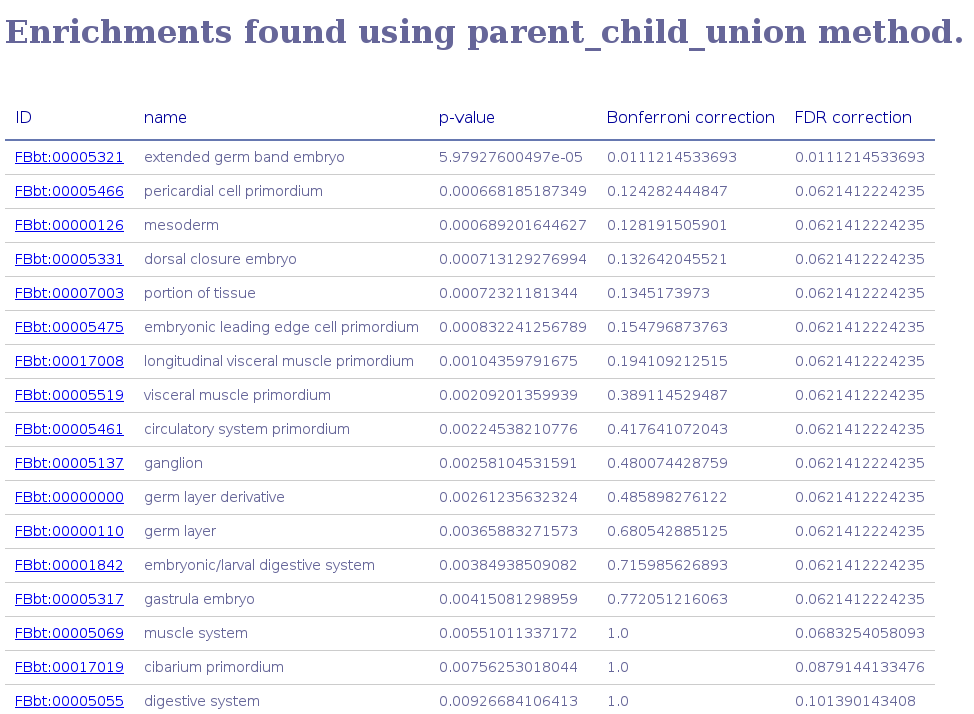
\includegraphics[width=0.8\textwidth]{images/pretty_print_html.png}
\caption{Enrichment representation as html.}
\label{fig:prettyhtml}
\end{figure}
\end{latexonly}

\item \verb|"tabular"| - writes enrichment results to tab-separated csv file, which
contain same columns as html output
\end{itemize}

\begin{thebibliography}{99}
\bibitem{cock2009}
Peter J. A. Cock, Tiago Antao, Jeffrey T. Chang, Brad A. Chapman, Cymon J. Cox, Andrew Dalke, Iddo Friedberg, Thomas Hamelryck, Frank Kauff, Bartek Wilczynski, Michiel J. L. de Hoon: ``Biopython: freely available Python tools for computational molecular biology and bioinformatics''. {\it Bioinformatics} {\bf 25} (11), 1422--1423 (2009). \href{http://dx.doi.org/10.1093/bioinformatics/btp163}{doi:10.1093/bioinformatics/btp163},
\bibitem{chapman2000}
Brad Chapman and Jeff Chang: ``Biopython: Python tools for computational biology''. \textit{ACM SIGBIO Newsletter} {\bf 20} (2): 15--19 (August 2000).

\end{thebibliography}
\end{document}

